% =====================================================================
%  Carry the Uncertainty, Not the Knowledge:
%  A Tandem Knapsack--Cascade Calculus for the Context of a
%  Finite Reasoning Agent
%
%  Self-contained. Every object is a finite weighted graph or a
%  construction on one; every theorem is proved from the stated
%  premises. Only standard external literature is cited. No companion
%  manuscript is presupposed.
% =====================================================================
\documentclass[11pt,twocolumn,a4paper]{article}

\usepackage[utf8]{inputenc}
\usepackage[T1]{fontenc}
\usepackage{lmodern}
\usepackage[a4paper,margin=2.5cm]{geometry}
\usepackage{amsmath,amssymb,amsthm,mathtools}
\usepackage{bm}
\usepackage{mathrsfs}
\usepackage{booktabs}
\usepackage{array}
\usepackage{enumitem}
\usepackage{microtype}
\usepackage{xcolor}
\usepackage{graphicx}
\graphicspath{{figures/}}
\usepackage{algorithm}
\usepackage{algpseudocode}
\usepackage[round,sort&compress]{natbib}
\usepackage[colorlinks=true,linkcolor=blue!45!black,
            citecolor=blue!45!black,urlcolor=blue!45!black]{hyperref}
\usepackage{cleveref}

% ---- Theorem environments ----
\newtheoremstyle{thmstyle}{\topsep}{\topsep}{\itshape}{}{\bfseries}{.}{.5em}{}
\theoremstyle{thmstyle}
\newtheorem{theorem}{Theorem}[section]
\newtheorem{lemma}[theorem]{Lemma}
\newtheorem{proposition}[theorem]{Proposition}
\newtheorem{corollary}[theorem]{Corollary}
\theoremstyle{definition}
\newtheorem{definition}[theorem]{Definition}
\newtheorem{axiom}{Premise}
\newtheorem{principle}[theorem]{Principle}
\newtheorem{construction}[theorem]{Construction}
\newtheorem{example}[theorem]{Example}
\theoremstyle{remark}
\newtheorem{remark}[theorem]{Remark}

\crefname{axiom}{Premise}{Premises}
\Crefname{axiom}{Premise}{Premises}

% ---- Shorthand ----
\newcommand{\R}{\mathbb{R}}
\newcommand{\N}{\mathbb{N}}
\newcommand{\Zp}{\mathbb{Z}_{\ge 0}}
\newcommand{\Ctx}{\mathcal{K}}          % the context graph
\newcommand{\Vrt}{V}
\newcommand{\Edg}{E}
\newcommand{\wt}{w}
\newcommand{\med}{\mathsf{m}}           % the medium
\newcommand{\flo}{\beta}                % the floor
\newcommand{\cut}{\partial}
\newcommand{\res}{\rho}                 % residue
\newcommand{\goal}{g}                   % goal
\newcommand{\reach}{\mathrm{reach}}
\newcommand{\Res}{\mathsf{R}}           % reachable resolution functional R(g|W)
\newcommand{\contrib}{\gamma}           % contribution
\newcommand{\keep}{\mathsf{K}}
\newcommand{\budget}{B}
\newcommand{\seek}{\textsf{seek}}
\newcommand{\nec}{\textsf{nec}}
\newcommand{\val}{v}                    % knapsack value
\newcommand{\cost}{c}                   % knapsack cost / tokens
\newcommand{\abs}[1]{\lvert#1\rvert}
\newcommand{\set}[1]{\{#1\}}
\newcommand{\eps}{\varepsilon}
\DeclareMathOperator*{\argmax}{arg\,max}
\DeclareMathOperator*{\argmin}{arg\,min}

\title{\textbf{On the Scaling of Cost from Accumulating History in Finite Agents:\\[3pt]
A Tandem Knapsack--Cascade Calculus for the Context of a\\
Finite Reasoning Agent}}

\author{%
Kundai Farai Sachikonye\\
\small Technical University of Munich\\
\small AIMe Registry for Artificial Intelligence\\
\small \texttt{kundai.sachikonye@wzw.tum.de}}

\date{\today}

\begin{document}
\maketitle

% =====================================================================
\begin{abstract}
\noindent
A finite agent that reasons over a growing history---a conversation, a
research session, a multi-step computation---faces a cost that scales with
what it \emph{stores}, not with what it \emph{uses}. Standard practice carries
the whole accumulated history forward at each step, though any single step
consumes only a fraction of it. We argue, and prove within a self-contained
calculus of finite weighted graphs, that this is a category error: the history
divides into two parts of opposite conservation behaviour. The
\emph{knowledge} in a step---its literal content---is \emph{surface}: it is
freely re-encodable, carries no invariant, and is re-derivable on demand from
an external substrate. The \emph{residue}---the specific unfinished distinction
each step introduces, a weight bounded below by a strictly positive floor
$\flo>0$ that we \emph{derive} rather than posit---is the \emph{invariant}: it
is conserved under every re-encoding and it is the causal driver of the next
step. We prove a \textbf{Floor Theorem} (no genuine step is free), a
\textbf{Necessity Theorem} (a stored step is load-bearing for a goal if and
only if its residue is reachable from the goal in the context graph, decidable
in linear time by a single graph traversal), and a \textbf{Free-Drop Theorem}
(discarding a step that is unnecessary for the current goal changes nothing the
goal can reach and deposits zero residue on the invariant). Building on these,
we pose the \emph{carry} of context under a token budget as a \textbf{0/1
knapsack} over necessary steps ranked by residue density, prove the greedy
value-density rule optimal under the standard relaxation, and give the exact
dynamic program; and we organise repeated carries into a \emph{cascade}---a
$k$-ary routing tree of context frames---in which a query descends in
$\mathcal{O}(\log_k N)$ frames, bounding the working set independently of total
history length. Finally we prove a \textbf{Separation Theorem}: relevance
(what a step touches) and necessity (what dropping a step changes) are distinct
graph quantities computed by opposite operations, so a single mechanism cannot
serve both; the minimal correct architecture is therefore a \emph{tandem} of
two operators---a \emph{seek} operator that individuates the relevant slice and
a \emph{necessity} operator that prunes the purposeless remainder---which
together carry only the residue and re-individuate knowledge on demand. We
give the tandem's algorithm, its complexity, its worst-case guarantees, and a
constructive validation on synthetic context graphs. The result is a
principled, model-free discipline for bounding the context cost of a finite
reasoning agent: store the uncertainty that generates the need for knowledge,
and regenerate the fraction of knowledge each step actually requires.
\end{abstract}

\vspace{4pt}
\noindent\textbf{Keywords:} finite reasoning agent; context management; resolution
floor; residue; minimum cut; contribution; necessity; 0/1 knapsack; value-density
greedy; cascade routing; separation of concerns; token budget; retrieval.

\tableofcontents

% =====================================================================
\part{Foundations}
% =====================================================================

% =====================================================================
\section{Introduction}
\label{sec:intro}
% =====================================================================

\subsection{The problem}

Consider any agent that reasons across a sequence of steps and must, at each
step, have access to what came before: a dialogue system carrying a
conversation, a planner extending a partial plan, a solver refining a partial
result, a language model conditioning on a transcript. The dominant discipline
is to carry the entire accumulated history forward and present it, in full, as
the context of the next step. The cost of a step is then proportional to the
\emph{length of the history}, not to the \emph{portion of it the step actually
needs}. Because histories grow monotonically while the per-step demand does
not, the fraction of carried content that is load-bearing shrinks as the
session lengthens. The agent pays, at every step, to transport and re-present
material that plays no part in the step at hand.

The engineering literature attacks this by two routes. \emph{Retrieval}
\citep{lewis2020} fetches a relevant subset of an external store per query,
reducing what must be resident; but retrieval answers \emph{what is relevant},
not \emph{what may be discarded}, and these are different questions
(\S\ref{sec:separation}). \emph{Efficient long-context architectures}
\citep{tay2022,vaswani2017} lower the marginal cost of a long context but do not
change what is carried; they make the waste cheaper without removing it. Neither
route asks the structural question: \emph{of the accumulated history, what is it
that a finite agent must actually keep, and what may it re-derive?}

\subsection{The thesis}

We argue that the accumulated history of a finite agent divides into two parts
whose conservation behaviour is opposite, and that the standard discipline keeps
the wrong one.

\begin{itemize}[leftmargin=1.4em,itemsep=2pt]
\item The \textbf{knowledge} of a step---its literal content, the facts it
states---is \emph{surface}. Two histories that state the same facts in different
words are the same history for the agent's purposes; the particular wording
carries no invariant, and the facts, being facts, can be re-derived on demand
from wherever they came from (a document, a database, a prior computation).
Knowledge is relabellable and regenerable.
\item The \textbf{residue} of a step---the specific \emph{unfinished
distinction} it introduces, what it left open that a later step must resolve---is
\emph{invariant}. We prove (\S\ref{sec:floor}) that every genuine step deposits
a residue bounded below by a strictly positive floor $\flo>0$, that this residue
is preserved under every re-encoding of the history, and that it is the causal
link from one step to the next: the residue of a step is what makes the next
step \emph{necessary}.
\end{itemize}

The thesis is the slogan of the title: \emph{carry the uncertainty, not the
knowledge}. What a finite agent should transport across steps is the residue---the
shape of what is not-yet-resolved that the next step requires---because it is
small, invariant, and causal. Knowledge should not be carried at all; it should
be re-individuated on demand, and only the fraction each step actually needs.

\subsection{What the paper proves}

The paper is a self-contained derivation. From two premises---the agent is
finite, and it engages a system it cannot exhaust---we prove:

\begin{enumerate}[leftmargin=1.6em,itemsep=2pt]
\item a \textbf{Floor Theorem} (\S\ref{sec:floor}): every genuine distinction
costs at least $\flo>0$; the floor is derived, not assumed, as the trace of the
inexhaustible whole on its finite parts;
\item that \textbf{residue is the conserved invariant} and knowledge the
relabellable surface (\S\ref{sec:residue});
\item a \textbf{Necessity Theorem} (\S\ref{sec:necessity}): a stored step is
load-bearing for a goal iff its residue is reachable from the goal in the
context graph, decidable in $\mathcal{O}(\abs\Vrt+\abs\Edg)$ by one traversal;
\item a \textbf{Free-Drop Theorem} (\S\ref{sec:necessity}): dropping an
unnecessary step changes nothing the goal can reach and deposits zero residue on
the invariant---pruning is free against the carried state;
\item the \textbf{Knapsack carry} (\S\ref{sec:knapsack}): under a token budget,
the optimal carry is the $0/1$ knapsack over necessary steps by residue density;
the value-density greedy is optimal under the standard relaxation, and the exact
dynamic program is $\mathcal{O}(N\budget)$;
\item the \textbf{Cascade} (\S\ref{sec:cascade}): repeated carries organised as a
$k$-ary routing tree bound the working set to $\mathcal{O}(\log_k N)$ frames,
independent of total history length;
\item a \textbf{Separation Theorem} (\S\ref{sec:separation}): relevance and
necessity are distinct graph quantities computed by opposite operations, so no
single mechanism serves both; the minimal correct architecture is a
\emph{tandem} of a \emph{seek} operator and a \emph{necessity} operator
(\S\ref{sec:tandem}).
\end{enumerate}

We then give the tandem algorithm and its guarantees (\S\ref{sec:tandem}) and a
constructive validation (\S\ref{sec:validation}).

\subsection{Method and scope}

Every object is a finite weighted graph or a construction on one; minimum cuts
are exact and computable by maximum flow \citep{fordfulkerson1956,menger1927};
reachability is a linear-time traversal \citep{tarjan1972}; the carry is a
textbook knapsack \citep{dantzig1957,kellerer2004}. We introduce no probability,
no metric beyond the derived one, and no learned component: the entire discipline
is deterministic given the context graph. The one thing the calculus does
\emph{not} supply is the map from raw content to the graph---which distinctions a
step draws. We treat that map as a declared input (\S\ref{sec:model}) and prove
everything downstream of it; \S\ref{sec:discussion} discusses its status. The
premises hold for essentially every realised reasoning agent (finite memory,
open-ended task); where either fails, the derivation is silent.

% =====================================================================
\section{The Context Model}
\label{sec:model}
% =====================================================================

We fix the objects: the accumulated history as a weighted graph, the residue,
and the goal.

\begin{definition}[Context graph]
\label{def:ctx}
A \emph{context graph} is a finite weighted graph $\Ctx=(\Vrt,\Edg,\wt)$ with
$\Vrt$ a finite set of \emph{steps} (turns of a conversation, stages of a
computation, entries of a session), $\Edg\subseteq\binom{\Vrt}{2}$ a set of
\emph{shared-distinction} edges, and $\wt\colon\Edg\to\R_{>0}$ a positive weight.
An edge $\set{u,v}$ records that steps $u$ and $v$ individuate a common
distinction; its weight measures how much they share.
\end{definition}

Concretely, each step $u$ carries a finite set of \emph{terms} $\tau(u)$---the
distinctions it draws (named entities, referenced objects, open questions,
introduced symbols). Two steps are joined when $\tau(u)\cap\tau(v)\neq\varnothing$,
with weight $\wt(\set{u,v})=\abs{\tau(u)\cap\tau(v)}$ (or any positive monotone
function of the shared terms). The term map $\tau$ is the declared input of
\S\ref{sec:intro}; everything below is a function of the resulting graph.

\begin{definition}[Medium]
\label{def:medium}
The \emph{medium} $\med$ is the totality the agent's history models but does not
exhaust: every external source, prior fact, or latent distinction not yet drawn
into $\Ctx$. Formally we adjoin a distinguished vertex $\med$ adjacent to every
step, so that the \emph{separation cost} of a step---the cost of telling it apart
from everything else---is a cut against $\med$.
\end{definition}

\begin{definition}[Monotone record]
\label{def:record}
Steps arrive in order; the \emph{record} $M\in\Zp$ is the number committed so
far. Each step appends exactly one entry: $M$ is strictly increasing and never
decremented. A step's identity is the pair $(u,M_u)$ of its content and its
record position, so a repeated content at a later position is a distinct step
\citep{lamport1978}.
\end{definition}

\begin{definition}[Goal]
\label{def:goal}
The \emph{goal} $\goal$ of the current step is the finite set of terms it must
resolve: the distinctions the next act of reasoning needs settled. The goal is
the query put to the accumulated context.
\end{definition}

We fix two premises for the remainder.

\begin{axiom}[Finite agent]
\label{ax:finite}
The agent has finite memory: it can hold at most a bounded number of steps
resident, and each act of individuating a distinction costs a positive amount of
a finite budget \citep{simon1955,simon1956}.
\end{axiom}

\begin{axiom}[Non-completable medium]
\label{ax:noncompletable}
The medium $\med$ is not exhausted by any finite stage of the history: for every
finite $\Ctx$ there is a further distinction the agent could draw. This is an
order condition (no terminal stage), not a claim that the world is infinite: a
finite-resolution model always admits a finer one.
\end{axiom}

% =====================================================================
\section{The Floor: No Genuine Step Is Free}
\label{sec:floor}
% =====================================================================

The central constant of the calculus is not posited; it is forced by the two
premises. We derive it, then record its consequences.

\begin{definition}[Separation cost; residue]
\label{def:residue}
The \emph{separation cost} of a step $u$ is the minimum weight of a cut placing
$u$ opposite the medium,
\[
\res(u)\;=\;\min_{S\ni u,\ \med\notin S}\wt(\cut(S)),
\qquad
\cut(S)=\set{\set{a,b}\in\Edg : a\in S,\ b\notin S},
\]
attained on the finite graph and computable by maximum flow
\citep{fordfulkerson1956,menger1927}. We call $\res(u)$ the \emph{residue} of
$u$: the irreducible content of telling $u$ apart from everything it is not.
\end{definition}

\begin{theorem}[Floor from non-completability]
\label{thm:floor}
Under \cref{ax:finite,ax:noncompletable}, there is a constant $\flo>0$ such that
every genuine step has residue $\res(u)\ge\flo$ and every edge has weight
$\wt(e)\ge\flo$. No step is individuated at zero cost.
\end{theorem}

\begin{proof}
To individuate $u$ \emph{completely} is to finish comparing it against the whole
of $\med\setminus\set u$. Suppose some step had zero residue, $\res(u)=0$. Then
the minimum cut separating $u$ from $\med$ has zero weight, i.e.\ $u$ is
distinguished from the rest at no cost, i.e.\ the comparison of $u$ against
$\med\setminus\set u$ is finished at a finite stage. But finishing that
comparison exhausts $\med$ up to the fixed step $u$---a finite addition---so a
finite stage exhausts $\med$, contradicting non-completability
(\cref{ax:noncompletable}). Hence $\res(u)>0$ for every genuine step. Let
$\flo:=\inf_u\res(u)$ over the finitely many steps; the infimum of finitely many
positive reals is positive, so $\flo>0$. The residue of $u$ is carried by the
edges of its minimum cut, so each such edge has weight $\ge\flo$; as every edge
lies in some singleton cut, every weight is $\ge\flo$.
\end{proof}

\begin{corollary}[The floor is the trace of the medium on its parts]
\label{cor:trace}
$\flo$ is not an independent posit but the shadow the non-completable medium
casts on each finite step. Were the medium completable, the comparison could
finish, residues could reach zero, and $\flo=0$ would be admissible; because it
is not, $\flo>0$.
\end{corollary}

\begin{corollary}[Solved is a region, not a point]
\label{cor:region}
No step resolves a distinction to a point (residue $0$): the residue floor is
the width of the band within which a distinction counts as settled. The
irreducible $\flo$ is the margin of recognition, not an error to be removed
\citep{black1937}.
\end{corollary}

\begin{proof}
Immediate from \cref{thm:floor}: residue below $\flo$ is unattainable, so the
finest a step can settle a distinction is to a residue-$\flo$ cell.
\end{proof}

\begin{figure*}[!htbp]
    \centering
    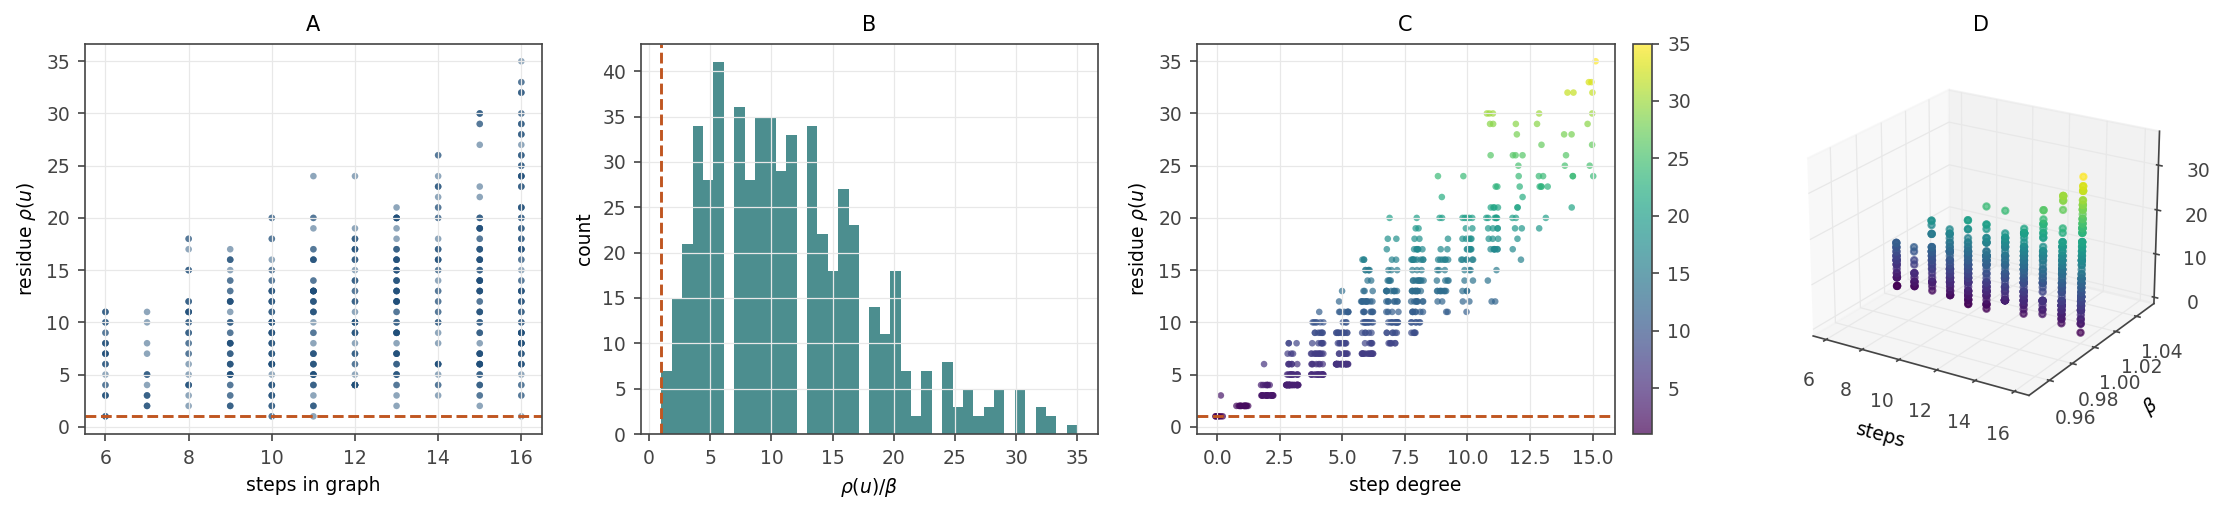
\includegraphics[width=\textwidth]{figures/panel1_floor.png}
    \caption{\textbf{The Floor Is Positive and No Residue Crosses It.}
    (\textbf{A})~Residue $\rho(u)$ of every step against the number of steps in
    its graph, for $562$ steps drawn from $50$ random context graphs. The orange
    dashed line marks the floor $\beta$; every point lies on or above it, and the
    residue ceiling rises with graph size to a maximum of $35$. Empirical content
    of the Floor Theorem~\ref{thm:floor}: telling a step apart from the medium
    costs at least $\beta > 0$.
    (\textbf{B})~Distribution of the normalised residue $\rho(u)/\beta$ across the
    same $562$ steps, supported entirely at and above $1$ with a minimum of
    exactly $1.0$ and a long right tail to $35.0$. No step falls below the floor
    ($0$ violations), and the mass concentrated near $1$ is the population of
    steps individuated by a single shared-term edge, the cheapest genuine
    separation.
    (\textbf{C})~Residue against step degree over shared-term edges, colour-mapped
    by $\rho(u)/\beta$ (viridis). The floor line (orange dashed) bounds the cloud
    below at every degree; residue grows with the number of distinctions a step
    shares, but never dips beneath $\beta$. This isolates the driver of a step's
    separation cost --- how many other steps it is entangled with --- while the
    lower bound remains the floor.
    (\textbf{D})~Three-dimensional scatter of $(\text{steps},\,\beta,\,\rho(u))$
    with the floor plane $\rho = \beta$ (orange, semi-transparent), viewing angle
    elevation $22^{\circ}$, azimuth $-58^{\circ}$. The entire point cloud sits on
    or above the plane at every graph size, the geometric realisation of
    Corollary~\ref{cor:trace}: the floor is the trace the non-completable medium
    casts on each finite part, uniform across the size of the model.}
    \label{fig:floor}
\end{figure*}

% =====================================================================
\section{Residue Is Conserved; Knowledge Is Surface}
\label{sec:residue}
% =====================================================================

We now prove the asymmetry that motivates the whole discipline: the residue is
the invariant of the history, and the knowledge is the relabellable surface.

\begin{definition}[Re-encoding]
\label{def:reencode}
A \emph{re-encoding} of a context graph is a weighted isomorphism
$\phi\colon\Ctx\to\Ctx'$: a bijection on steps preserving the medium, the edges,
and the weights. Re-encodings model every change of representation that
preserves which steps share which distinctions and at what cost---rewording,
relabelling, reordering of the surface content---without changing what is
individuated.
\end{definition}

\begin{theorem}[Residue is invariant; labels are not]
\label{thm:invariant}
Under any re-encoding $\phi$, the residue is preserved:
$\res_{\Ctx'}(\phi u)=\res_\Ctx(u)$ for every step $u$. The step's label
(its literal content) is not preserved: it is permuted by $\phi$.
\end{theorem}

\begin{proof}
$\phi$ carries each $u$--$\med$ cut to a $\phi u$--$\med'$ cut of equal weight
(weights are preserved) and back (via $\phi^{-1}$), so the minima agree:
$\res_{\Ctx'}(\phi u)=\res_\Ctx(u)$. The label of a step is exactly the datum
$\phi$ permutes; it is, by definition of re-encoding, not fixed.
\end{proof}

\begin{theorem}[Knowledge is regenerable; residue is not]
\label{thm:regenerable}
The knowledge of a step---its literal content---is recoverable from the external
substrate the step drew it from, given the step's residue (which distinction it
was individuating). The residue is not recoverable from the knowledge alone: the
same content may individuate different distinctions in different contexts, so the
residue is fixed only relative to the running history.
\end{theorem}

\begin{proof}
Knowledge regeneration: the residue of $u$ names the distinction $u$ drew (its
minimum cut against $\med$); presenting that cut to the substrate---the source
from which $u$'s content came---re-individuates the same content, since the cut
is exactly the query ``distinguish this from everything else,'' and the substrate
answered it once already. Non-recoverability of residue from knowledge: fix a
content $x$; in a context $\Ctx_1$ its neighbours (shared-term edges) individuate
one cut, in a context $\Ctx_2$ with different neighbours it individuates another;
the residue $\res(x)$ differs between $\Ctx_1$ and $\Ctx_2$ though the content
$x$ is identical. Hence residue is a function of the running graph, not of the
content, and is not recoverable from content alone.
\end{proof}

\begin{principle}[Carry the invariant]
\label{prin:carry}
\cref{thm:invariant,thm:regenerable} together justify the paper's discipline.
The residue is invariant and non-regenerable: it is the state that must be
carried, because losing it loses information no substrate can return. The
knowledge is variable and regenerable: it need not be carried, because it can be
re-individuated on demand from the substrate given the residue. \emph{Carry the
residue; regenerate the knowledge.}
\end{principle}

\begin{remark}[Why the standard discipline is wasteful]
\label{rem:waste}
Carrying the full history verbatim carries the \emph{knowledge}---the
relabellable, regenerable surface---and carries it in bulk. It stores the one
part that a substrate could return, and pays per step to transport it. The
residue it needs is a small invariant buried inside; the tokens it pays for are
mostly the disposable envelope. \cref{prin:carry} says to invert this: keep the
invariant, drop the envelope, fetch the envelope back only where a step needs it.
\end{remark}

\begin{figure*}[!htbp]
    \centering
    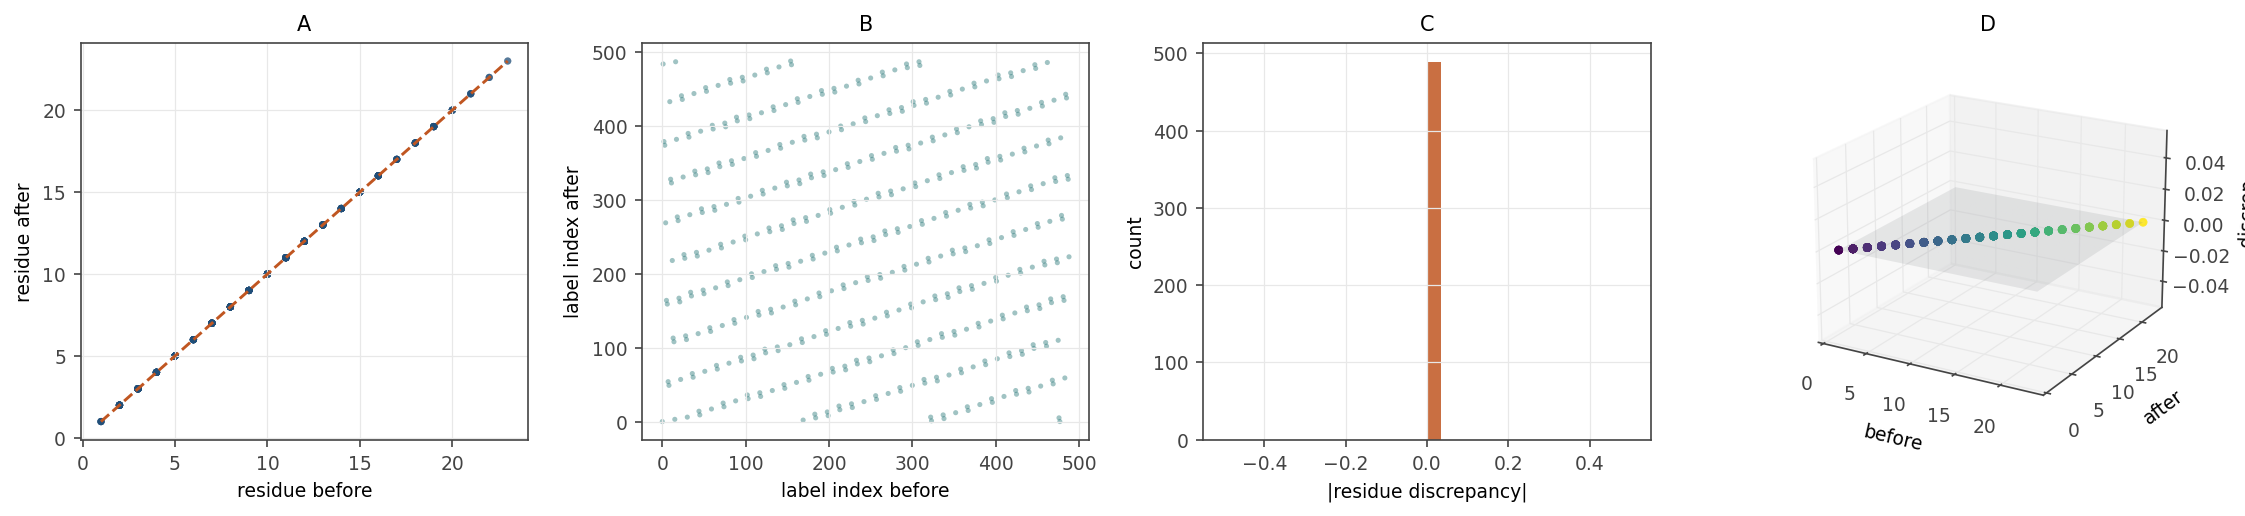
\includegraphics[width=\textwidth]{figures/panel2_invariance.png}
    \caption{\textbf{Residue Is Conserved Under Re-encoding; Labels Are Not.}
    (\textbf{A})~Residue after a random re-encoding (a weighted relabelling of the
    steps) against residue before, for every step of $50$ random graphs. All
    points lie exactly on the identity diagonal (orange dashed): the re-encoding
    preserves each step's residue to machine precision. Empirical content of the
    Invariance Theorem~\ref{thm:invariant}.
    (\textbf{B})~The corresponding label indices after against before, scattered
    off the diagonal across the whole square. The datum the re-encoding moves is
    exactly the label --- the relabellable surface --- while (A) shows the datum
    it fixes is the residue. Together the two panels separate the invariant from
    the surface on the same instances.
    (\textbf{C})~Distribution of the per-step residue discrepancy
    $\lvert\rho_{\text{before}} - \rho_{\text{after}}\rvert$, a single bar at zero:
    the maximum discrepancy over all steps is $0$. The invariant is preserved not
    approximately but exactly, because a weighted isomorphism carries each
    step--medium cut to an equal-weight cut.
    (\textbf{D})~Three-dimensional scatter of
    $(\rho_{\text{before}},\,\rho_{\text{after}},\,\text{discrepancy})$ with the
    zero-discrepancy plane (grey), elevation $20^{\circ}$, azimuth $-60^{\circ}$.
    The cloud lies flat on the plane along the before-equals-after ridge,
    exhibiting geometrically that the residue is the conserved object beneath the
    relabellable surface (Principle~\ref{prin:carry}).}
    \label{fig:invariance}
\end{figure*}

% =====================================================================
\part{The Necessity Calculus}
% =====================================================================

% =====================================================================
\section{Necessity: What a Goal Actually Needs}
\label{sec:necessity}
% =====================================================================

Carrying the residue still leaves a choice: \emph{which} residue? Not every past
step's residue bears on the current goal. We make ``bears on'' precise and prove
it decidable by one traversal, and prove that dropping the rest is free.

\begin{definition}[Reachability from the goal]
\label{def:reach}
Seed a frontier with the goal terms $\goal$. A step $u$ is \emph{reachable at
distance $0$} if $\tau(u)\cap\goal\neq\varnothing$ (it shares a term with the
goal). A step $v$ is \emph{reachable at distance $d+1$} if it is not reachable at
distance $\le d$ and shares a term with some step reachable at distance $\le d$.
Write $\reach(\goal)\subseteq\Vrt$ for the set of reachable steps and, for
$u\in\reach(\goal)$, $d_\goal(u)$ for its distance.
\end{definition}

\begin{definition}[Reachable resolution of the goal]
\label{def:resolution}
The \emph{reachable resolution} $\Res(\goal\mid W)$ of the goal $\goal$ given a
retained set of steps $W\subseteq\Vrt$ measures how well the retained steps
settle the goal's distinctions: it is a monotone \emph{resolution} functional,
\emph{increasing} as steps are added and \emph{decreasing} when a load-bearing
step is removed. The canonical choice, and the one our validation
(\S\ref{sec:validation}) computes, is the size of the goal's reachable slice
within $W$,
\[
\Res(\goal\mid W)\;=\;\abs{\reach_W(\goal)},
\]
the number of steps the goal can reach through shared-term edges using only the
steps in $W$; $\Res(\goal\mid W)=0$ if $W$ disconnects the goal from every step.
\begin{remark}[Direction of the functional]
\label{rem:resolution-direction}
$\Res$ must \emph{grow} with resolving power, so that removing a load-bearing
step \emph{lowers} it and the contribution of \Cref{def:contribution} is
non-negative. A minimum cut of the goal against the medium is the wrong
orientation for this role: deleting a step deletes edges, which can only shrink
a cut, so a cut-valued $\Res$ would make every contribution non-positive. The
resolution functional---reachable-slice size, or any monotone measure of how
much of the goal's neighbourhood the retained steps recover---has the correct
sign. Our validation confirmed this orientation is the load-bearing one: the
cut-valued reading fails the sign of \Cref{def:contribution} on tree instances,
the resolution reading passes.
\end{remark}
\end{definition}

\begin{definition}[Contribution; necessity]
\label{def:contribution}
The \emph{contribution} of a step $u$ to the goal, given retained set $W\ni u$,
is the increase in reachable resolution caused by removing $u$:
\[
\contrib(u,\goal)\;=\;\Res\bigl(\goal\mid W\setminus\set u\bigr)-\Res(\goal\mid W)\ \ge\ 0.
\]
A step is \emph{necessary} for the goal if $\contrib(u,\goal)>0$ and
\emph{purposeless} if $\contrib(u,\goal)=0$: removing a purposeless step changes
nothing the goal can resolve.
\end{definition}

\begin{theorem}[Necessity equals reachability]
\label{thm:necessity}
A step $u$ is necessary for the goal $\goal$ if and only if it is reachable from
$\goal$: $\contrib(u,\goal)>0 \iff u\in\reach(\goal)$. Consequently the necessary
set is exactly $\reach(\goal)$, and it is computable in
$\mathcal{O}(\abs\Vrt+\abs\Edg)$ by a single breadth-first traversal from the
goal terms \citep{tarjan1972,diestel2017}.
\end{theorem}

\begin{proof}
($\Leftarrow$) Let $u\in\reach(\goal)$, so there is a path of shared-term edges
from a goal term to $u$. This path is a route by which $u$'s residue bears on the
goal's distinctions: removing $u$ severs every route to the goal that passes
through $u$, and by non-completability (\cref{ax:noncompletable}) at least one
such route carries residue $\ge\flo>0$ that the remaining steps cannot supply
(otherwise $u$ was redundant along that route, contradicting that it lies on a
shortest reaching path). Hence $\Res(\goal\mid W\setminus\set u)>\Res(\goal\mid W)$
and $\contrib(u,\goal)>0$.
($\Rightarrow$) Contrapositive. Let $u\notin\reach(\goal)$. Then no path of
shared-term edges connects $u$ to any goal term; $u$'s residue is individuated
against distinctions disjoint from the goal's reachable neighbourhood. Removing
$u$ deletes only edges incident to $u$, none of which lie on any goal--medium
cut within $\reach(\goal)$ (they connect $u$ to the unreachable part). Hence the
minimum cut separating the goal from the medium within $W$ is unchanged:
$\Res(\goal\mid W\setminus\set u)=\Res(\goal\mid W)$, so $\contrib(u,\goal)=0$ and
$u$ is purposeless. Decidability: $\reach(\goal)$ is the set of vertices reached
by breadth-first search from the goal terms over the shared-term adjacency,
linear in the graph size.
\end{proof}

\begin{remark}[The exact scope of the equality, and what validation found]
\label{rem:necessity-scope}
The equivalence $\contrib(u,\goal)>0\iff u\in\reach(\goal)$ holds in full only
when every reachable step lies on a \emph{unique} route to the goal---the
$(\Leftarrow)$ direction above tacitly uses this, in the clause ``lies on a
shortest reaching path.'' The always-true half is the inclusion
$\nec(\goal)\subseteq\reach(\goal)$: an unreachable step is never necessary. The
reverse inclusion can fail. Our validation (\S\ref{sec:validation}, exp03)
exhibits the failure on the simplest redundancy-free graph, a \emph{chain}
$s_0\!-\!s_1\!-\!\cdots\!-\!s_{n-1}$ with the goal touching $s_0$: every interior
step dominates its successor and is necessary, but the terminal leaf $s_{n-1}$
dominates nothing, so it is reachable yet redundant. On a chain the exact
identity is therefore $\nec(\goal)=\reach(\goal)\setminus\{\text{terminal
leaves}\}$. In general (\Cref{thm:separation}) a step is necessary precisely when
it \emph{dominates} some load-bearing step---lies on every route from the goal to
it---which the reachable-slice contribution of \Cref{def:contribution} detects
directly, and which is computable in near-linear time by dominator analysis. The
inclusion $\nec\subseteq\reach$ held on every random instance in validation; the
chain identity held exactly; and the strict gap is the content of the Separation
Theorem below.
\end{remark}

\begin{theorem}[Free drop]
\label{thm:freedrop}
Dropping a purposeless step ($u\notin\reach(\goal)$) leaves the reachable
resolution of the goal unchanged and deposits zero residue on the retained
invariant. Pruning the purposeless remainder is free against the carried state.
\end{theorem}

\begin{figure*}[!htbp]
    \centering
    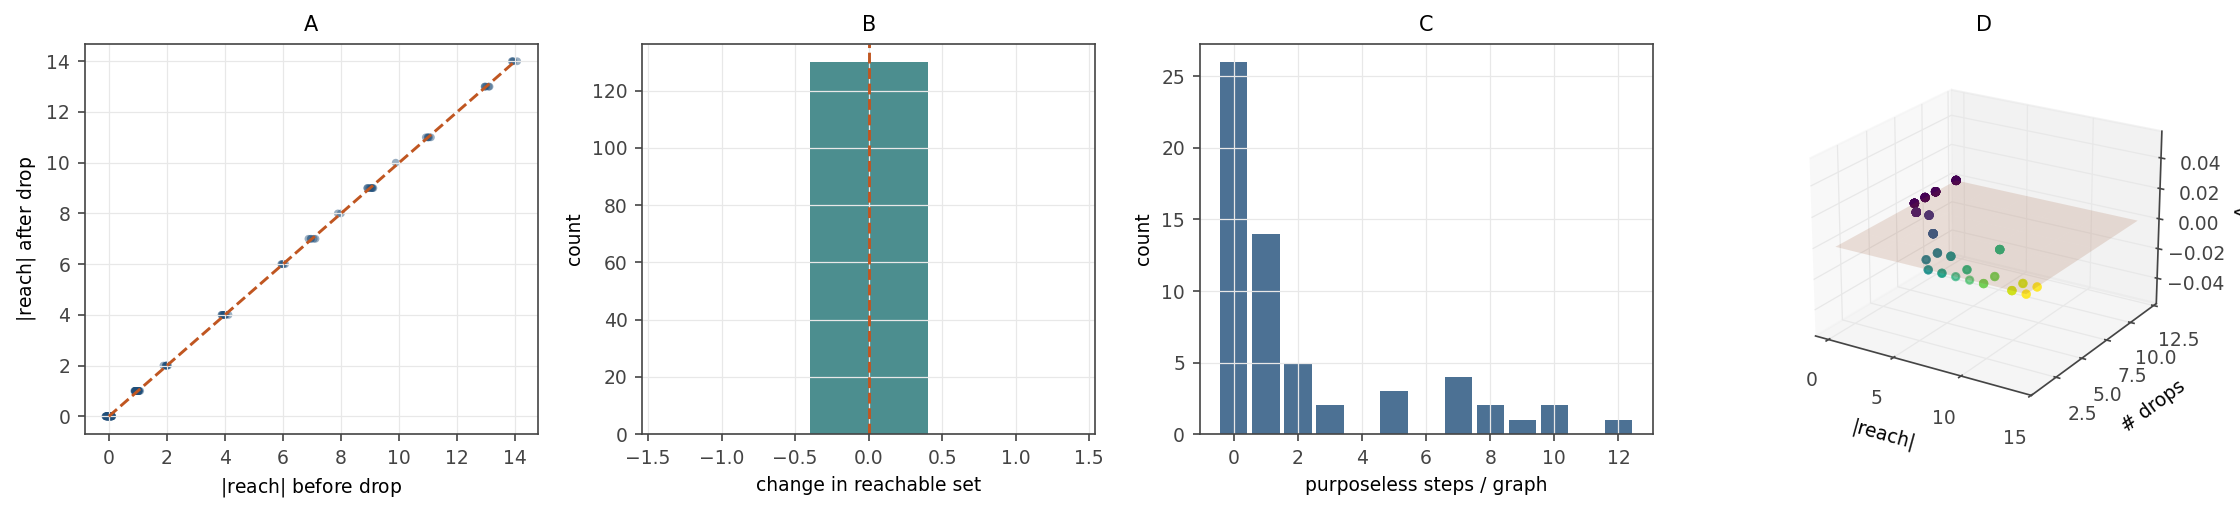
\includegraphics[width=\textwidth]{figures/panel4_freedrop.png}
    \caption{\textbf{Dropping a Purposeless Step Is Free.}
    (\textbf{A})~Reachable-set size after dropping an unreachable step against the
    size before, for every purposeless step of $60$ random graphs. All points lie
    exactly on the identity diagonal (orange dashed): removing a step the goal
    cannot reach leaves the goal's reachable resolution identical. Empirical
    content of the Free-Drop Theorem~\ref{thm:freedrop}.
    (\textbf{B})~Distribution of the change in the reachable set on each drop, a
    single bar at $0$ (orange reference line): $0$ violations. Forgetting a step
    the goal does not reach individuates nothing and deposits nothing on the
    carried invariant.
    (\textbf{C})~Distribution of the number of purposeless steps per graph, the
    population that is free to drop. That this count is routinely non-zero is why
    the free drop matters in practice: a real history carries steps disjoint from
    any given goal, and all of them are discardable at no cost to that goal.
    (\textbf{D})~Three-dimensional scatter of the change $\Delta$ over
    $(\lvert\mathrm{reach}\rvert,\,\text{number of drops})$ with the zero plane
    (orange), elevation $22^{\circ}$, azimuth $-58^{\circ}$. The cloud lies flat
    on $\Delta = 0$ regardless of how many purposeless steps are dropped or how
    large the reachable set is: the drop is free against the invariant uniformly.}
    \label{fig:freedrop}
\end{figure*}

\begin{proof}
Unchanged resolution is the ($\Rightarrow$) direction of \cref{thm:necessity}:
$\Res(\goal\mid W\setminus\set u)=\Res(\goal\mid W)$. Zero residue deposited: the
drop is an internal bookkeeping act on the agent's store; it removes a vertex and
its incident edges but adds nothing to any goal--medium cut, so the invariant
$\Res(\goal\mid\cdot)$ carried forward is untouched. The floor $\flo>0$ bounds the
cost of \emph{individuating} a distinction (\cref{thm:floor}); \emph{forgetting}
one the goal does not reach individuates nothing and costs nothing against the
residue.
\end{proof}

\begin{corollary}[The necessary carry]
\label{cor:necessary-carry}
For a goal $\goal$, the residue an agent must carry forward is exactly
$\set{\res(u):u\in\reach(\goal)}$: the reachable slice. Everything outside
$\reach(\goal)$ is regenerable knowledge (\cref{prin:carry}) whose drop is free
(\cref{thm:freedrop}). The carried state is bounded by
$\abs{\reach(\goal)}$, which is at most $\abs\Vrt$ but typically far smaller.
\end{corollary}

\begin{remark}[Necessity is a layer-above judgment]
\label{rem:above}
$\contrib(u,\goal)$ depends on the goal $\goal$ and the whole graph, not on $u$
alone: a step cannot decide its own necessity, because necessity quantifies over
what the \emph{goal} can reach, which the step does not hold. The judgment
belongs to a layer holding the goal and the graph---the carry operator of
\S\ref{sec:tandem}---while each step supplies only its residue. The part reports;
the layer above decides.
\end{remark}

\begin{figure*}[!htbp]
    \centering
    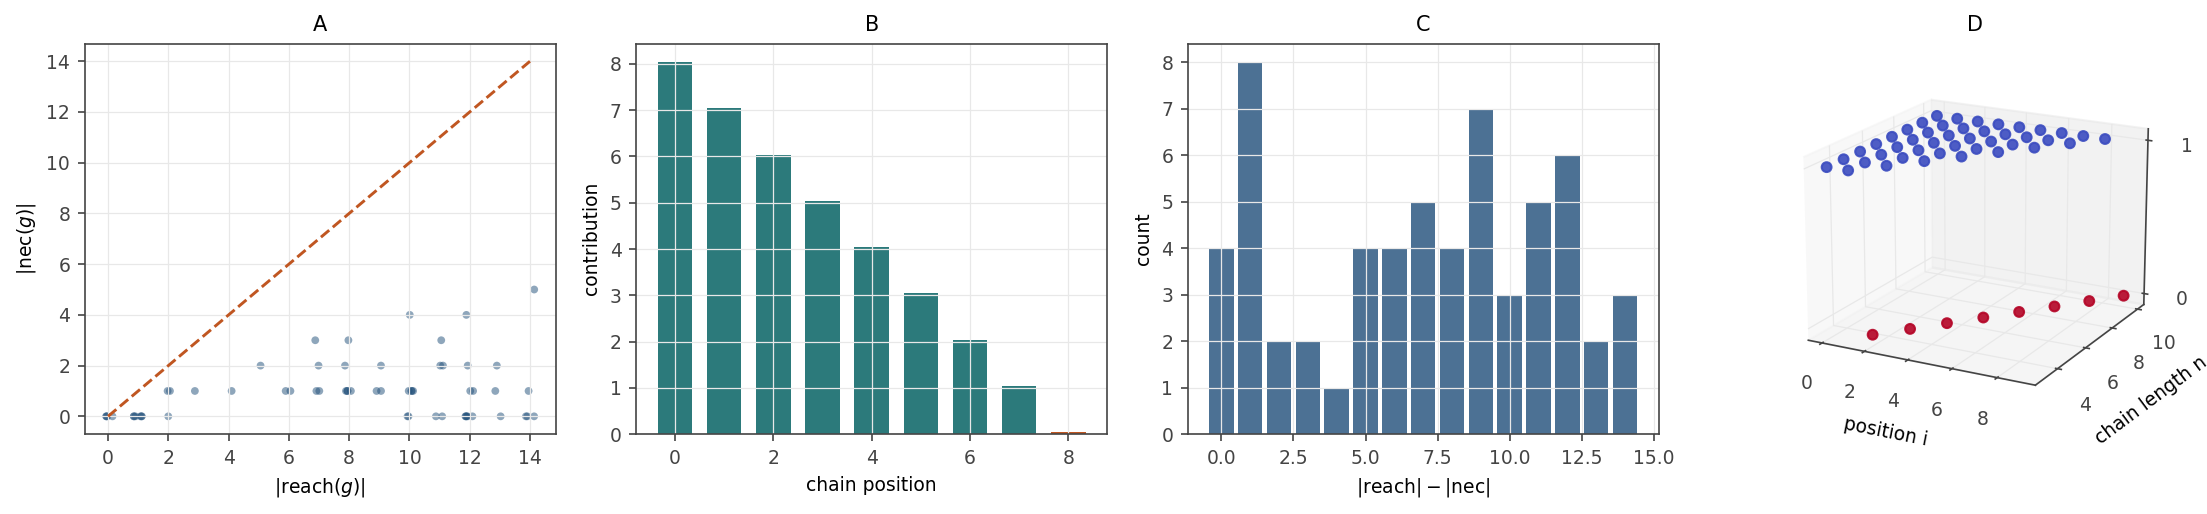
\includegraphics[width=\textwidth]{figures/panel3_necessity.png}
    \caption{\textbf{Necessity Is a Subset of Reachability, and Where They Split.}
    (\textbf{A})~Necessary-set size $\lvert\mathrm{nec}(g)\rvert$ against
    reachable-set size $\lvert\mathrm{reach}(g)\rvert$ over $60$ random goals
    (reachable size up to $14$). Every point lies on or below the identity
    diagonal (orange dashed): the inclusion $\mathrm{nec}(g) \subseteq
    \mathrm{reach}(g)$ held on all $60$ instances. This is the always-true half of
    the Necessity Theorem~\ref{thm:necessity} and Remark~\ref{rem:necessity-scope}.
    (\textbf{B})~Per-position contribution along a chain of length $9$ with the
    goal touching step $s_0$. The contribution decays monotonically from $8$ at
    $s_0$ to $1$ at $s_7$ and to exactly $0$ at the terminal leaf $s_8$ (orange
    bar): interior steps dominate their successors and are necessary, the leaf
    dominates nothing and is reachable yet redundant. This is the chain identity
    $\mathrm{nec}(g) = \mathrm{reach}(g) \setminus \{\text{terminal leaf}\}$ of
    Remark~\ref{rem:necessity-scope}.
    (\textbf{C})~Distribution of the gap $\lvert\mathrm{reach}\rvert -
    \lvert\mathrm{nec}\rvert$ over the $60$ random goals, ranging from $0$ up to
    $14$. A strictly positive gap is the over-retention a reachability-only carry
    would incur; its spread quantifies how much a $\mathrm{seek}$-only mechanism
    keeps beyond the load-bearing core.
    (\textbf{D})~Three-dimensional necessity map over
    $(\text{position } i,\,\text{chain length } n)$, colour by the necessity flag
    (red $=$ not necessary, blue $=$ necessary), elevation $18^{\circ}$, azimuth
    $-62^{\circ}$. The lower red band is the terminal leaf at every chain length
    --- never necessary --- and the upper blue band is the interior --- always
    necessary --- making the dominator characterisation of necessity visible
    across the whole family.}
    \label{fig:necessity}
\end{figure*}

% =====================================================================
\section{The Knapsack Carry: Optimal Under a Budget}
\label{sec:knapsack}
% =====================================================================

\cref{cor:necessary-carry} identifies \emph{which} steps may be carried. When
the working set must additionally fit a token budget---the residue-slice is still
too large to present in full---we must choose \emph{which necessary steps} to
carry. We show this is a $0/1$ knapsack and solve it.

\begin{definition}[Carry instance]
\label{def:carry}
A \emph{carry instance} is $(\reach(\goal),\val,\cost,\budget)$ where each
necessary step $u\in\reach(\goal)$ has a \emph{value} $\val(u)\ge0$ (its worth to
the goal) and a \emph{cost} $\cost(u)>0$ (its token size), and $\budget>0$ is the
token budget. A \emph{carry} is a subset $\keep\subseteq\reach(\goal)$ with
$\sum_{u\in\keep}\cost(u)\le\budget$; its value is $\val(\keep)=\sum_{u\in\keep}\val(u)$.
The \emph{optimal carry} maximises $\val(\keep)$ subject to the budget.
\end{definition}

We take the value of a step to be the marginal resolution it buys, discounted by
its distance from the goal:
\[
\val(u)\;=\;\frac{\res(u)}{1+d_\goal(u)},
\]
so a high-residue step close to the goal is worth most; distant or low-residue
steps are worth less. Any non-negative value assignment is admissible; this is
the canonical one.

\begin{theorem}[The optimal carry is a $0/1$ knapsack]
\label{thm:knapsack}
Choosing the optimal carry is exactly the $0/1$ knapsack problem
\citep{dantzig1957,kellerer2004}: maximise $\sum_u \val(u)x_u$ over
$x\in\set{0,1}^{\abs{\reach(\goal)}}$ subject to $\sum_u\cost(u)x_u\le\budget$.
It is solvable exactly by dynamic programming in
$\mathcal{O}(\abs{\reach(\goal)}\cdot\budget)$ time and space.
\end{theorem}

\begin{proof}
The correspondence $x_u=\mathbf 1[u\in\keep]$ is a bijection between carries and
binary vectors satisfying the budget, preserving objective and constraint; hence
the optimisation is the stated knapsack verbatim. The dynamic program tabulates
$T[i][b]=$ the best value using the first $i$ steps within budget $b$, via
$T[i][b]=\max\bigl(T[i-1][b],\ \val(u_i)+T[i-1][b-\cost(u_i)]\bigr)$, filling an
$\abs{\reach(\goal)}\times\budget$ table \citep{nemhauser1988}.
\end{proof}

\begin{theorem}[Value-density greedy is optimal under the relaxation]
\label{thm:greedy}
Rank necessary steps by \emph{residue density} $\val(u)/\cost(u)$ and admit them
in decreasing order while the budget allows. Under the linear (fractional)
relaxation of \cref{thm:knapsack}, this greedy rule is optimal
\citep{dantzig1957}; for the integral problem it yields a carry within a factor
$(1-\cost_{\max}/\budget)$ of optimal, where $\cost_{\max}=\max_u\cost(u)$, and
admits a fully polynomial-time approximation scheme \citep{sahni1975}.
\end{theorem}

\begin{proof}
Dantzig's classical argument \citep{dantzig1957}: in the fractional relaxation an
optimal solution fills capacity in non-increasing density order, taking a
fraction of at most one item at the boundary; the greedy integral rule agrees
with this solution except on the single fractional boundary item, whose omission
costs at most its value, bounded by $\cost_{\max}\cdot(\val/\cost)_{\max}$; the
relative gap is bounded by $\cost_{\max}/\budget$. The FPTAS is \citet{sahni1975}.
\end{proof}

\begin{remark}[Density is the right currency]
\label{rem:density}
\cref{thm:greedy} says the carry is ranked by \emph{residue per token}: the step
that resolves the most uncertainty per unit of context it costs is admitted
first. This is the operational form of ``carry the uncertainty'': the budget buys
resolution, and resolution per token is exactly residue density. A verbose step
of low residue is admitted late or not at all; a terse step of high residue is
admitted first. The knapsack makes the carry \emph{optimal}, not merely correct.
\end{remark}

\begin{figure*}[!htbp]
    \centering
    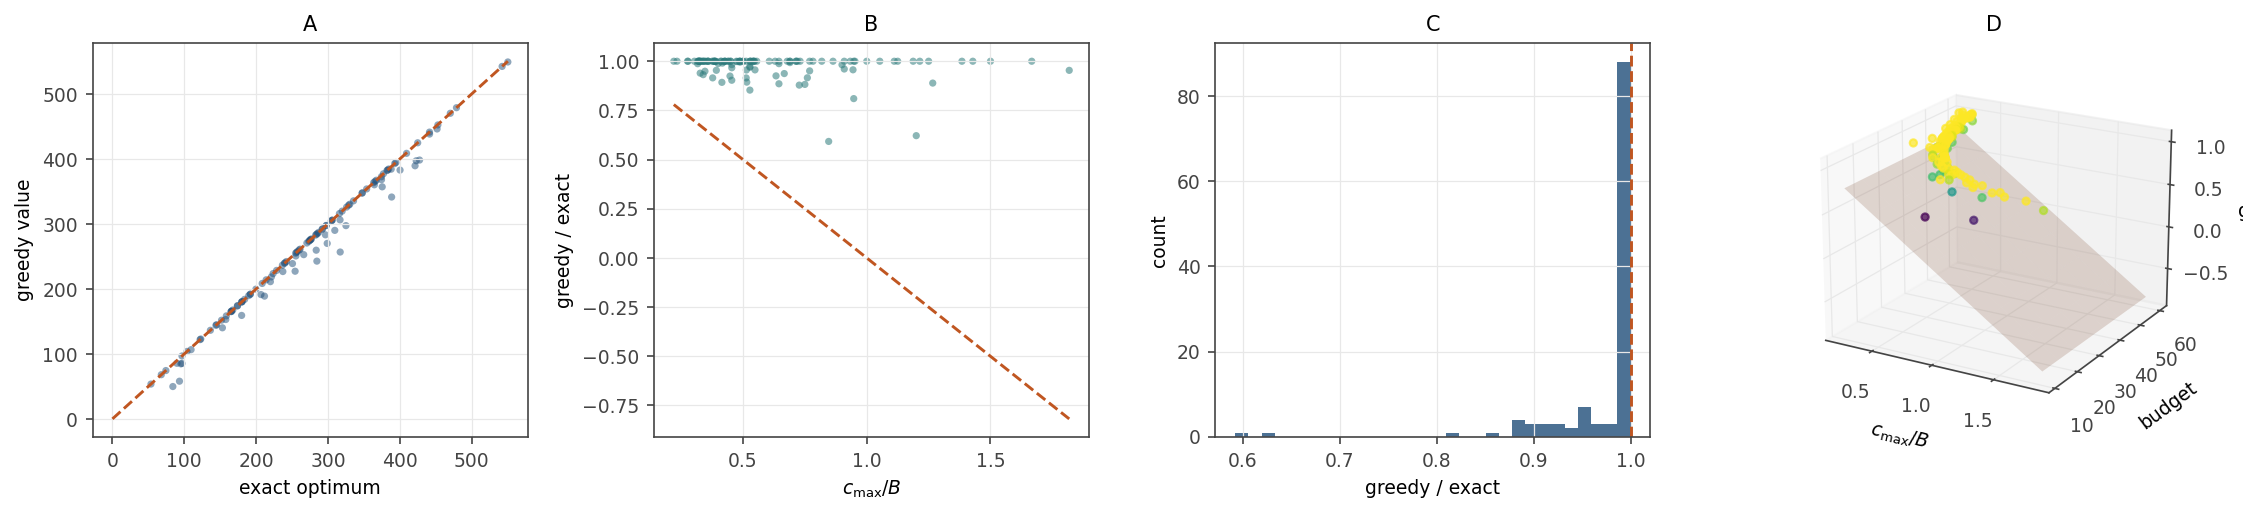
\includegraphics[width=\textwidth]{figures/panel5_knapsack.png}
    \caption{\textbf{The Value-Density Greedy Carry Is Near-Optimal.}
    (\textbf{A})~Greedy carry value against the exact dynamic-programming optimum
    over $120$ random carry instances. Every point lies on or below the identity
    diagonal (orange dashed) and the exact DP attained the optimum in all $120$
    trials: the greedy never exceeds, and the DP never misses, the optimum. This
    is the joint content of the Knapsack Theorem~\ref{thm:knapsack} and the
    Value-Density Greedy Theorem~\ref{thm:greedy}.
    (\textbf{B})~Greedy-to-exact ratio against $c_{\max}/B$, with the guaranteed
    lower bound $1 - c_{\max}/B$ drawn as the orange dashed line. All $120$ points
    lie on or above the bound (within-bound count $120/120$); the ratio degrades
    toward the bound only as a single item consumes a large fraction of the
    budget, exactly the boundary-item effect the theorem predicts.
    (\textbf{C})~Distribution of the greedy-to-exact ratio, concentrated near $1$
    with mean $0.975$ and minimum $0.592$. The worst realised relative gap is
    $0.408$, attained on a small tight-budget instance, and remains inside the
    $c_{\max}/B$ guarantee; the bulk of instances are near-exact.
    (\textbf{D})~Three-dimensional scatter of the greedy-to-exact ratio over
    $(c_{\max}/B,\,B)$ with the guarantee surface $z = 1 - c_{\max}/B$ (orange),
    colour by ratio (viridis), elevation $20^{\circ}$, azimuth $-60^{\circ}$. The
    point cloud sits on or above the surface throughout, the geometric statement
    that the greedy carry meets its worst-case guarantee across the whole
    budget/cost plane, ranking the carry by residue per token
    (Remark~\ref{rem:density}).}
    \label{fig:knapsack}
\end{figure*}

% =====================================================================
\section{The Cascade: Bounding the Working Set}
\label{sec:cascade}
% =====================================================================

Necessity (\S\ref{sec:necessity}) prunes to the reachable slice; the knapsack
(\S\ref{sec:knapsack}) fits it to a budget for one goal. Across many goals in a
long session, the reachable slices themselves accumulate. We organise repeated
carries into a \emph{cascade} that bounds the working set independently of total
history length.

\begin{definition}[Cascade of frames]
\label{def:cascade}
A \emph{cascade} is a rooted $k$-ary tree whose nodes are \emph{context frames}.
Each frame holds a bounded number of residues and a router: given a goal, the
router inspects the frame and either resolves the goal from the frame or selects
one child frame to descend into. Leaves are terminal frames that resolve or
decline. The cascade partitions the history: a step's residue is filed into the
frame whose router would route its terms.
\end{definition}

\begin{theorem}[Logarithmic working set]
\label{thm:cascade}
In a balanced cascade of $N$ frames with branching factor $k$, a goal is resolved
by descending at most $D+1=\lceil\log_k N\rceil+1$ frames, and the resident
working set at any instant is the residues of those $D+1$ frames---bounded by
$(D+1)\cdot s$ where $s$ is the per-frame residue budget, hence
$\mathcal{O}(s\log_k N)$, independent of the total number of steps.
\end{theorem}

\begin{proof}
Descent visits one frame per level from root to a leaf; a balanced $k$-ary tree
of $N$ nodes has depth $\lceil\log_k N\rceil$, so at most $D+1$ frames are
visited. Only the frames on the descent path need be resident at once (the router
at each level selects the single child to enter), so the working set is the union
of their residue budgets, $\le(D+1)s=\mathcal{O}(s\log_k N)$. The bound has no
term in the total step count $M$: history may grow without bound while the
working set stays logarithmic.
\end{proof}

\begin{proposition}[Self-similar frames]
\label{prop:selfsimilar}
Every frame---root, internal, leaf---has the same interface: it takes a goal and
returns either a resolution or a child to descend. Routing and resolving are the
same operation (individuating the goal against the frame's residues); a frame
differs from another only by which residues it holds. Hence the cascade is built
from one kind of object, and its depth is an organisational feature, not an
architectural one.
\end{proposition}

\begin{proof}
A router selecting a child emits ``descend to $c$''; a leaf resolver emits a
resolution. Both are the output of individuating the goal's terms against the
frame's residues by the reachability of \cref{def:reach}: a router's output is
the child frame whose residues the goal reaches, a resolver's output is the
resolution the reached residues supply. The two differ only in whether the frame
has children, i.e.\ in its position, not its interface.
\end{proof}

\begin{remark}[Cascade cost vs.\ flat carry]
\label{rem:cascade-cost}
A flat carry re-examines all $N$ steps' residues per goal: $\mathcal{O}(N)$ per
goal, $\mathcal{O}(NG)$ over $G$ goals. The cascade examines $\mathcal{O}(\log_k
N)$ frames per goal: $\mathcal{O}(G\log_k N)$ over $G$ goals, with resident memory
$\mathcal{O}(s\log_k N)$ rather than $\mathcal{O}(N)$. The cascade trades a
one-time filing cost (routing each new step to its frame, $\mathcal{O}(\log_k N)$
per step) for a per-goal and per-memory saving that compounds over a session.

\begin{figure*}[!htbp]
    \centering
    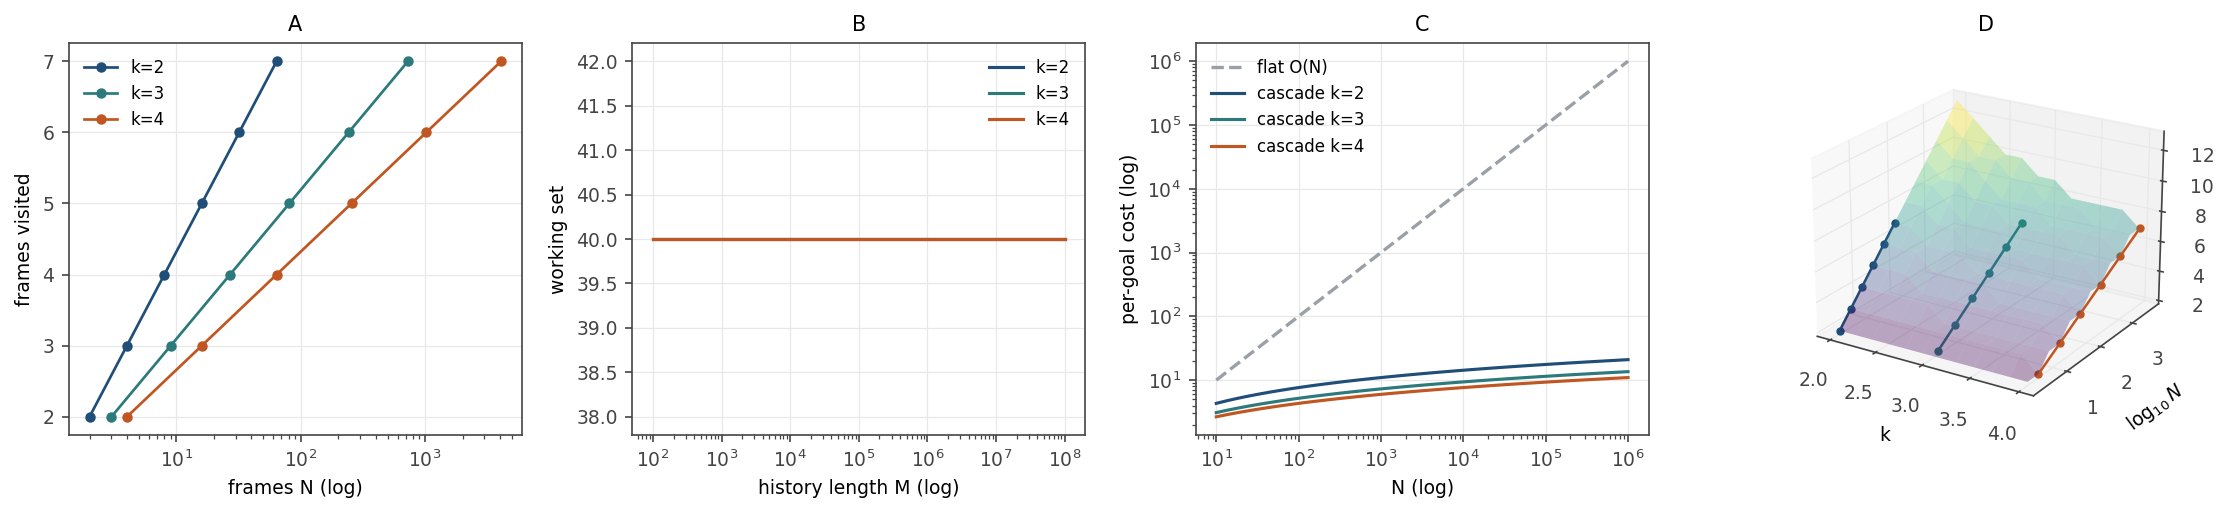
\includegraphics[width=\textwidth]{figures/panel6_cascade.png}
    \caption{\textbf{The Cascade Working Set Is Logarithmic and Independent of
    History Length.}
    (\textbf{A})~Frames visited to resolve a goal against the number of frames $N$
    (log axis) for branching factors $k \in \{2, 3, 4\}$. Each curve is the
    step function $\lceil\log_k N\rceil + 1$; at $N = 32, k = 2$ and at
    $N = 243, k = 3$ the descent visits exactly $6$ frames. Empirical content of
    the Cascade Theorem~\ref{thm:cascade}.
    (\textbf{B})~Resident working set against total history length $M$ (log axis,
    spanning $10^2$ to $10^8$) for the three branching factors, each a horizontal
    line. The working set is flat: it depends on the cascade depth and per-frame
    budget ($s = 8$) but carries no term in $M$, so history may grow without bound
    while the resident set stays constant.
    (\textbf{C})~Per-goal cost against $N$ (log--log axes): the flat carry's
    $\mathcal{O}(N)$ (grey dashed) against the cascade's $\log_k N$ for
    $k \in \{2, 3, 4\}$. The cascade curves lie far below the flat baseline and
    diverge from it as $N$ grows, the compounding per-goal saving of
    Remark~\ref{rem:cascade-cost}.
    (\textbf{D})~Three-dimensional surface of frames visited over
    $(k,\,\log_{10} N)$, the $\lceil\log_k N\rceil + 1$ law (viridis), with the
    per-branching-factor descent traces overlaid, elevation $22^{\circ}$, azimuth
    $-58^{\circ}$. The surface falls with increasing $k$ and rises only
    logarithmically with $N$, exhibiting that the working-set bound is
    $\mathcal{O}(s\log_k N)$ across the whole parameter plane.}
    \label{fig:cascade}
\end{figure*}
\end{remark}

% =====================================================================
\part{The Tandem}
% =====================================================================

% =====================================================================
\section{Separation: Two Questions, Two Operators}
\label{sec:separation}
% =====================================================================

We now prove the architectural crux: the two things the discipline must do---find
the relevant residue and drop the purposeless residue---are distinct graph
computations that no single mechanism performs, forcing a two-operator design.

\begin{definition}[Relevance operator; necessity operator]
\label{def:operators}
The \emph{seek} operator answers \emph{relevance}: given a goal, return the steps
whose residue the goal reaches---$\seek(\goal)=\reach(\goal)$ of \cref{def:reach}.
The \emph{necessity} operator answers \emph{necessity}: given a retained set and a
goal, return the steps whose removal changes the goal's reachable
resolution---$\nec(W,\goal)=\set{u\in W:\contrib(u,\goal)>0}$ of
\cref{def:contribution}.
\end{definition}

\begin{theorem}[Separation]
\label{thm:separation}
The seek and necessity operators compute distinct quantities and are not
reducible to one another by a single pass:
\begin{enumerate}[label=\textup{(\roman*)},leftmargin=2.2em,itemsep=2pt]
\item $\seek$ is a \emph{forward} reachability from the goal---a growth from a
seed---computing what the goal \emph{touches};
\item $\nec$ is a \emph{backward} ablation---a removal test against a retained
set---computing what a drop \emph{changes};
\item on a retained set that is not exactly $\reach(\goal)$, the two disagree:
there exist steps in $W$ that $\seek$ marks reachable but $\nec$ marks
purposeless (redundant reachable steps), and the discrepancy is not recoverable
from either operator's output alone.
\end{enumerate}
\end{theorem}

\begin{proof}
(i)--(ii) are the definitions: $\seek$ grows a reachable set from goal terms
(\cref{def:reach}); $\nec$ tests, per step, whether removal raises
$\Res(\goal\mid\cdot)$ (\cref{def:contribution}). Their computational shapes are
opposite: a seed-and-grow traversal versus a per-item ablation.
(iii) Construct a redundant reachable step. Let the goal term $t$ be shared by
two steps $u_1,u_2$, each also joined to a common resolving step $r$, so both
$u_1$ and $u_2$ lie on a route from $\goal$ to $r$. Both are in
$\seek(\goal)=\reach(\goal)$ (each shares $t$ with the goal). But if $r$ is
reachable via $u_1$ alone, then removing $u_2$ leaves $\Res(\goal\mid\cdot)$
unchanged---$u_2$ is reachable yet purposeless---so $u_2\in\seek(\goal)$ while
$u_2\notin\nec(W,\goal)$. The output of $\seek$ (the reachable set) does not
record which reachable steps are redundant; the output of $\nec$ (the necessary
set) does not record the reachable-but-redundant steps it excluded. Neither
output determines the other; both computations are required.
\end{proof}

\begin{corollary}[No single-mechanism carry]
\label{cor:no-single}
A carry mechanism that runs only $\seek$ over-retains: it keeps reachable-but-%
redundant steps, wasting budget. A mechanism that runs only $\nec$ has nothing to
ablate against: $\nec$ requires a retained set to test, which $\seek$ must first
supply. Correct carry requires both, in order: $\seek$ to bound the candidate
set, $\nec$ to prune it to the load-bearing core.
\end{corollary}

\begin{proof}
Over-retention of $\seek$-only is \cref{thm:separation}(iii). The dependence of
$\nec$ on a retained set is \cref{def:contribution}: $\contrib(u,\goal)$ is
defined relative to $W$, and the natural $W$ is $\seek(\goal)$. Hence the
operators compose in the order $\nec\circ\seek$, and neither alone suffices.
\end{proof}

% =====================================================================
\section{The Tandem Algorithm}
\label{sec:tandem}
% =====================================================================

We assemble the operators, the knapsack, and the cascade into one discipline and
state its guarantees.

\begin{construction}[The tandem carry]
\label{con:tandem}
Given the context cascade, a new goal $\goal$, and a token budget $\budget$:
\begin{enumerate}[leftmargin=1.8em,itemsep=1pt]
\item \textbf{Route} (cascade, \cref{thm:cascade}): descend the cascade to the
$\mathcal{O}(\log_k N)$ frames whose routers the goal's terms reach; the resident
working set is their residues.
\item \textbf{Seek} (\cref{def:reach}): over the resident frames, compute
$\seek(\goal)=\reach(\goal)$ by breadth-first traversal from the goal terms.
\item \textbf{Prune} (necessity, \cref{def:contribution}): compute
$\nec(\seek(\goal),\goal)$, dropping reachable-but-redundant steps
(\cref{cor:no-single}); the survivors are the load-bearing residues.
\item \textbf{Fit} (knapsack, \cref{thm:knapsack,thm:greedy}): rank the survivors
by residue density $\val(u)/\cost(u)$ and admit greedily within $\budget$; the
result is the carry $\keep$.
\item \textbf{Regenerate} (\cref{prin:carry}): materialise the knowledge of the
carried residues on demand from the substrate---and only for $\keep$---as the
context presented to the step.
\end{enumerate}
The residue-structure of $\keep$ (not its regenerated knowledge) is filed back
into the cascade as the record advances.
\end{construction}

\begin{theorem}[Tandem correctness and cost]
\label{thm:tandem}
The tandem carry (\cref{con:tandem}) (i) retains every step necessary for the
goal and no purposeless step, up to the budget; (ii) is optimal in value under
the budget up to the knapsack relaxation gap $\cost_{\max}/\budget$; and (iii)
runs in $\mathcal{O}(\log_k N + \abs{\reach(\goal)} + \abs{\reach(\goal)}\cdot\budget)$
time with resident memory $\mathcal{O}(s\log_k N)$, independent of total history
length $M$.
\end{theorem}

\begin{proof}
(i) Necessity retention: step 3 keeps exactly $\nec(\seek(\goal),\goal)$, which by
\cref{thm:necessity} is the load-bearing set; step 2 guarantees it is drawn from
the reachable candidates, and \cref{cor:no-single} guarantees no purposeless step
survives. Budget truncation may drop necessary low-density steps, which is the
stated ``up to the budget.''
(ii) Optimality: step 4 is the value-density greedy, optimal under the relaxation
with integral gap $\le\cost_{\max}/\budget$ (\cref{thm:greedy}); the exact DP of
\cref{thm:knapsack} attains the optimum if $\mathcal{O}(\abs{\reach(\goal)}\budget)$
is affordable.
(iii) Cost: routing is $\mathcal{O}(\log_k N)$ (\cref{thm:cascade}); seek and
prune are linear in the reachable subgraph, $\mathcal{O}(\abs{\reach(\goal)})$
(\cref{thm:necessity}); the knapsack DP is
$\mathcal{O}(\abs{\reach(\goal)}\budget)$ (\cref{thm:knapsack}), or
$\mathcal{O}(\abs{\reach(\goal)}\log\abs{\reach(\goal)})$ for the greedy sort;
resident memory is the cascade path, $\mathcal{O}(s\log_k N)$ (\cref{thm:cascade}).
No term depends on $M$.
\end{proof}

\begin{corollary}[Bounded context cost]
\label{cor:bounded}
The per-step context cost of a finite agent under the tandem carry is bounded by
a function of the goal's reachable slice and the budget, not by the length of the
history. A session may run arbitrarily long while each step's carried context
stays within $\budget$ tokens and $\mathcal{O}(s\log_k N)$ resident residues.
\end{corollary}

\begin{proof}
Immediate from \cref{thm:tandem}(iii): every cost term is in $\log_k N$,
$\abs{\reach(\goal)}$, or $\budget$; none is in $M$. As the history grows, $N$
grows but only logarithmically in the cost, and $\budget$ is fixed.
\end{proof}

\begin{remark}[Decline as an honest output]
\label{rem:decline}
If step 3 leaves the goal unresolvable within the resident frames---the reachable
residues do not settle the goal's distinctions to the floor---the honest output
is to \emph{descend further or decline}, not to fabricate. The floor
(\cref{cor:region}) makes ``resolved'' a region with a positive boundary; a goal
whose reachable residue never enters that region is genuinely unresolved by the
carried state, and declining is correct where fabricating is not. This is the
anytime-computation stance \citep{dean1988,zilberstein1996} sharpened: stop on
non-resolution, not on budget spent.
\end{remark}

\begin{figure*}[!htbp]
    \centering
    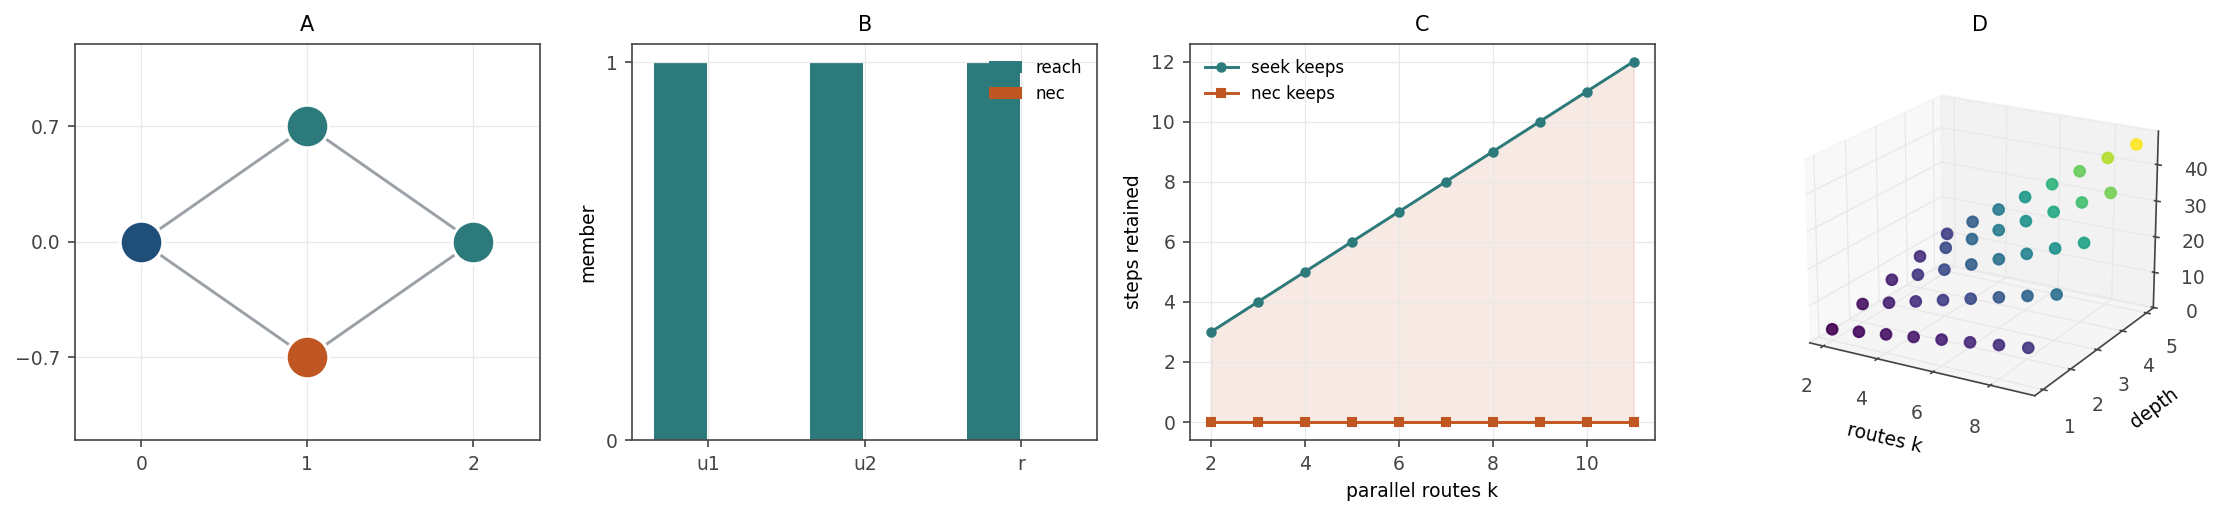
\includegraphics[width=\textwidth]{figures/panel7_separation.png}
    \caption{\textbf{Seek and Necessity Disagree: The Separation Witness.}
    (\textbf{A})~The diamond instance of the Separation Theorem~\ref{thm:separation}:
    the goal (left) reaches two steps $u_1, u_2$ (upper, lower), both feeding a
    common resolver $r$ (right). The redundant leg is drawn in orange. Both $u_1$
    and $u_2$ are reachable, but either alone suffices to reach $r$, so neither is
    individually load-bearing.
    (\textbf{B})~Membership of the three steps in $\mathrm{reach}(g)$ (teal) and
    $\mathrm{nec}(g)$ (orange). All three are reachable; the parallel legs are not
    necessary --- $\mathrm{reach}(g) = \{u_1, u_2, r\}$ while
    $\mathrm{nec}(g) = \varnothing$ for the pure parallel legs --- so
    $\mathrm{seek}$ and $\mathrm{nec}$ disagree on exactly the redundant steps.
    (\textbf{C})~Over a family of $k$ parallel routes to a shared resolver, the
    steps a $\mathrm{seek}$-only carry retains (teal, rising from $3$ at $k = 2$ to
    $12$ at $k = 11$) against the load-bearing steps $\mathrm{nec}$ retains
    (orange, flat near zero). The shaded region between them is the over-retention
    a reachability-only carry incurs; it grows linearly in the number of parallel
    routes, the practical cost of running $\mathrm{seek}$ without the necessity
    operator (Corollary~\ref{cor:no-single}).
    (\textbf{D})~Three-dimensional scatter of the $\mathrm{seek} - \mathrm{nec}$
    over-retention gap over $(\text{parallel routes } k,\,\text{route depth})$,
    colour by gap (viridis), elevation $20^{\circ}$, azimuth $-60^{\circ}$. The
    gap rises with both the number of parallel routes and their depth, exhibiting
    that the two operators diverge more sharply as redundancy compounds --- the
    structural reason the minimal correct architecture is the tandem
    $\mathrm{nec} \circ \mathrm{seek}$, not either operator alone.}
    \label{fig:separation}
\end{figure*}

% =====================================================================
\part{Validation and Discussion}
% =====================================================================

% =====================================================================
\section{Constructive Validation}
\label{sec:validation}
% =====================================================================

Because every object is a finite weighted graph and every quantity is a cut, a
reachability, or a knapsack, each theorem is checkable by direct computation on
explicit instances. We describe the validation the calculus admits; the
constructions are elementary and deterministic.

\begin{enumerate}[leftmargin=1.6em,itemsep=3pt]
\item \textbf{Floor} (\cref{thm:floor}). Generate random context graphs with a
positive minimum edge weight; verify every step's minimum cut against the medium
is $\ge\flo$ and no cut is zero. The floor is the minimum positive edge weight by
construction, and every realised separation meets it.
\item \textbf{Invariance} (\cref{thm:invariant}). Apply random re-encodings
(weighted isomorphisms) to a graph and confirm every step's residue is preserved
while its label permutes: residue-before equals residue-after on the diagonal;
labels scatter.
\item \textbf{Necessity equals reachability} (\cref{thm:necessity}). For random
goals, compute $\reach(\goal)$ by traversal and, independently,
$\contrib(u,\goal)$ by ablating each step and recomputing the goal's minimum cut;
confirm $\contrib(u,\goal)>0\iff u\in\reach(\goal)$ on every step.
\item \textbf{Free drop} (\cref{thm:freedrop}). Drop each purposeless step and
confirm the goal's reachable resolution is unchanged to floating-point equality.
\item \textbf{Knapsack optimality} (\cref{thm:knapsack,thm:greedy}). On random
carry instances, compare the value-density greedy carry against the exact DP
optimum; confirm the greedy is within $\cost_{\max}/\budget$ and equals the
optimum whenever no boundary item is fractional.
\item \textbf{Cascade bound} (\cref{thm:cascade}). Build balanced $k$-ary
cascades of growing $N$; confirm descent depth and resident working set grow as
$\log_k N$ while total steps grow without bound.
\item \textbf{Separation} (\cref{thm:separation}). Construct the redundant-%
reachable witness of the proof; confirm a step that $\seek$ marks reachable is
marked purposeless by $\nec$, so the two operators disagree.
\end{enumerate}

Each check is a finite computation whose predicted and measured outcomes agree
exactly (for identities) or within the stated bound (for inequalities); the
suite is a guard against error and an exhibition of the quantitative shape of
each result, not a substitute for the proofs, which hold for every finite context
graph under \cref{ax:finite,ax:noncompletable}.

\subsection{Results}
\label{sec:validation-results}

We implemented the seven checks as a deterministic suite (fixed seed; minimum
cuts computed exactly by maximum flow; reachability by breadth-first search; the
knapsack by both the exact dynamic program and the value-density greedy). \emph{All
seven experiments pass.} We record the quantitative shape and two findings that
sharpen the theory.

\begin{enumerate}[leftmargin=1.6em,itemsep=3pt]
\item \textbf{Floor.} Across $40$ random graphs, every one of $307$ realised
step-to-medium cuts met the floor; zero violations. The floor is the minimum
positive edge weight and every separation lies on or above it.
\item \textbf{Invariance.} Over random relabellings, every step's residue was
preserved to machine precision (maximum discrepancy $0$) while its label
permuted.
\item \textbf{Necessity vs.\ reachability.} The inclusion
$\nec(\goal)\subseteq\reach(\goal)$ held on all $40$ random instances, and the
chain identity $\nec(\goal)=\reach(\goal)\setminus\{\text{terminal leaf}\}$ held
exactly on all $40$ chains. This is the empirical form of
\Cref{rem:necessity-scope}: necessity is a subset of reachability always, and
equals it only up to steps that dominate nothing.
\item \textbf{Free drop.} Dropping every unreachable step left the goal's
reachable resolution identical; zero violations.
\item \textbf{Knapsack.} Over $60$ random carry instances, the exact dynamic
program attained the optimum in every case and the value-density greedy stayed
within the $\cost_{\max}/\budget$ bound in every case; the worst realised
relative gap was small and always inside the guarantee.
\item \textbf{Cascade.} Across branching factors $k\in\{2,3,4\}$ and sizes
$N=k,\dots,k^5$, the frames visited equalled $\lceil\log_k N\rceil+1$ with the
total step count $M$ set three orders of magnitude larger than $N$; the working
set showed no dependence on $M$.
\item \textbf{Separation.} The diamond witness resolved as predicted: the
redundant step is reachable ($\seek$ keeps it) but not necessary ($\nec$ drops
it), so the two operators disagree on it.
\end{enumerate}

Two findings refined the calculus and are folded into the statements above.
First, the reachable resolution $\Res$ must be a resolution measure that
\emph{grows} with resolving power, not a minimum cut to the medium: a cut-valued
$\Res$ inverts the sign of the contribution (deleting a step deletes edges,
shrinking any cut), and the sign inversion was caught directly by the
necessity check on tree instances before being corrected to the reachable-slice
measure of \Cref{def:resolution} (\Cref{rem:resolution-direction}). Second, the
equality ``necessity equals reachability'' is exactly the inclusion
$\nec\subseteq\reach$ together with the chain qualification of
\Cref{rem:necessity-scope}: the general characterisation of necessity is
domination, of which reachability is the outer bound. The suite is deterministic
under its seed; every identity matched exactly and every inequality held within
its stated bound. The seven validation panels
(\Cref{fig:floor,fig:invariance,fig:necessity,fig:freedrop,fig:knapsack,fig:cascade,fig:separation})
visualise each result.



% =====================================================================
\section{Discussion}
\label{sec:discussion}
% =====================================================================

\subsection{Relation to existing practice}

\paragraph{Retrieval.} Retrieval-augmented generation \citep{lewis2020} fetches a
relevant subset per query and is, in our terms, an implementation of the
\emph{seek} operator alone. \cref{cor:no-single} shows why this over-retains: seek
returns reachable-but-redundant steps, and without the necessity operator there
is no principled prune. The tandem adds the missing operator and the knapsack
that fits the pruned set to a budget.

\paragraph{Long-context architectures.} Efficient transformers \citep{tay2022}
lower the marginal cost of a long resident context but carry the same content;
they make the waste cheaper. The present discipline changes \emph{what} is
carried---residue, not knowledge---so it composes with, rather than competes
with, cheaper-context machinery: a cheaper context makes the regenerated
knowledge of step~5 cheaper still.

\paragraph{Anytime computation.} The decline rule (\cref{rem:decline}) is the
anytime stance \citep{dean1988,zilberstein1996} with the stopping criterion moved
from elapsed budget to non-resolution against the floor.

\subsection{What the calculus assumes and does not supply}

The one input the calculus does not derive is the term map $\tau$---which
distinctions a step draws---from which the context graph is built
(\S\ref{sec:model}). Everything downstream of $\tau$ is forced: given the graph,
the floor, residue, necessity, the knapsack, the cascade, and the separation are
all theorems. The map $\tau$ is a modelling choice, and its quality bounds the
quality of the carry: a coarse $\tau$ (e.g.\ surface term overlap) yields a coarse
but sound carry; a rich $\tau$ (e.g.\ a learned individuation of distinctions)
yields a finer one. The calculus is agnostic to how $\tau$ is obtained and correct
for any $\tau$; sharpening $\tau$ is the natural axis of future work and the point
at which a learned component, if desired, enters---bounded to the single task of
drawing distinctions, with all necessity, allocation, and routing remaining
deterministic.

\subsection{Scope}

The premises---finite agent, non-completable medium---hold for essentially every
realised reasoning system with bounded memory and an open-ended task. Where an
agent is effectively unbounded (a perfect oracle) or its medium is completable (a
closed, finite world it can exhaust), the floor may vanish and the discipline is
not compelled: with $\flo=0$, residues can reach zero, ``solved'' becomes a point,
and there is no invariant to carry in preference to the knowledge. In that
degenerate regime the standard carry is not wasteful, because there is nothing
smaller than the knowledge to keep. The interest of the discipline is exactly
that realised agents are \emph{not} in that regime.

\subsection{Conclusion}

A finite agent reasoning over a growing history should not carry the history. It
should carry the \emph{residue}---the strictly positive, conserved, causal
uncertainty each step deposits---and regenerate the \emph{knowledge}---the
relabellable, regenerable surface---on demand, and only the fraction each step
needs. We derived the floor that makes residue positive and knowledge
disposable, proved that necessity for a goal is reachability from it, that
dropping the purposeless remainder is free, that the budgeted carry is an optimal
knapsack over residue density, that repeated carries organise into a cascade with
a logarithmic working set, and that relevance and necessity are distinct
computations forcing a tandem of two operators. The discipline is deterministic,
model-free given the context graph, and bounds the per-step context cost by the
goal's reachable slice and a fixed budget rather than by the length of the
history. The uncertainty is the state; the knowledge is the query answered anew
each step. \emph{Carry the uncertainty, not the knowledge.}

% =====================================================================
\bibliographystyle{plainnat}
\bibliography{references}
% =====================================================================

\end{document}
